\subsection{Aufbau}
\label{subsec:aufbau}

Im Folgenden soll die interne Architektur des \gls{go1} im Detail dargestellt werden.
Hierfür werden einige Perspektiven des Roboters gezeigt, um die nach Einsatzzweck klassifizierten Bauteilgruppen zu erläutern und darzustellen.

\subsubsection{Überblick}

Die zoomorphe Form des \gls{go1} ist - wie bereits mehrfach angedeutet - an die eines Hundes angelehnt.
So ergeben sich die Bezeichnungen der äußerlich erkennbaren Bauteile von selbst.
Abbildung~\ref{fig:allgemeine_architektur} zeigt die äußerlichen Merkmale im Überblick.

\begin{figure}[h]
    \frame{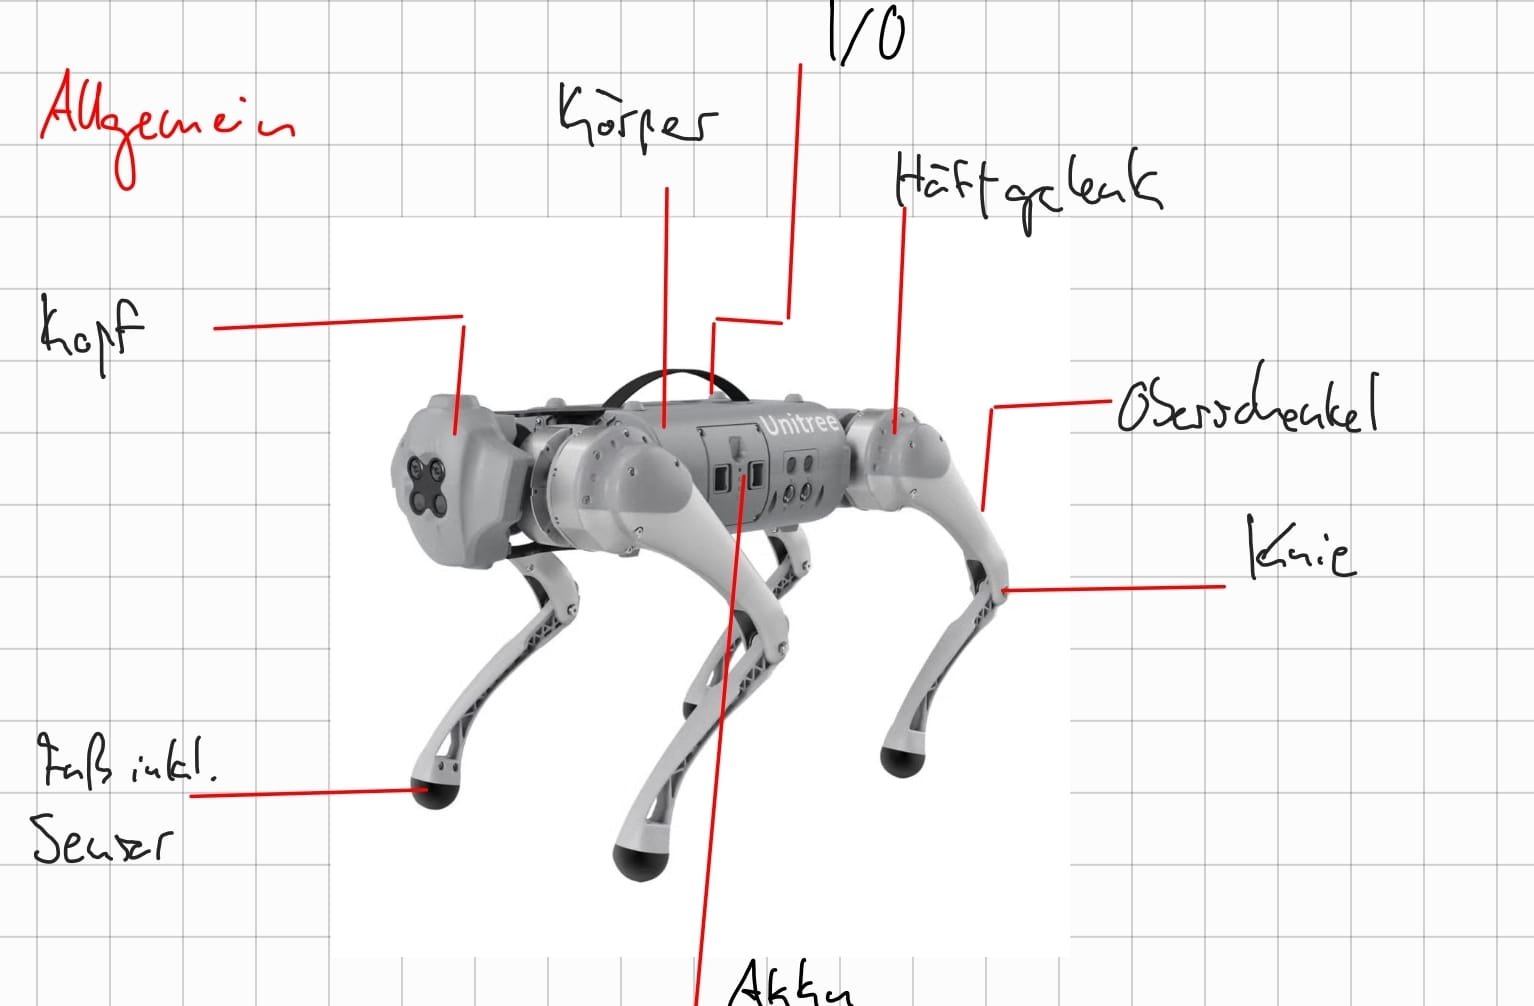
\includegraphics[width=\linewidth]{img/architektur/allgemein}}
    \caption[Überblick über den Go1]{Überblick über den \gls{go1}}\label{fig:allgemeine_architektur}
\end{figure}

Die Grundlage des Roboters bildet der Körper - auf Abbildung~\ref{fig:allgemeine_architektur} mit \numref{1} gekennzeichnet.
In diesem sind ie meisten Komponenten des \gls{go1} verbaut, unter Anderen die folgenden:
\begin{itemize}
    \item Interne Hardwarekomponenten
    \item Intelligenter Akku
    \item Teile der Sensorik und Kameras
    \item Hüftgelenke und Motoren der Beine
\end{itemize}
Eine genauere Beschreibung der Einzelteile findet sich in den folgenden Unterkapiteln.
An der Vorderseite des Körpers ist der Kopf \numref{2} des Roboters verbaut.
In diesem sind beispielsweise ein \emph{Nvidia Jetson Nano}, eine Stereo-Kamera und Stereo Ultraschall Sensoren
und weitere Bauteile wie Lautsprecher und Mikrofone verbaut.
An den vier äußeren Ecken des Körpers sind die Beine des Roboters verbaut.
Innerhalb des Körpers sind die Motoren zur Steuerung der Hüftgelenke \numref{3} integriert.
Außerhalb der Hüftgelenke an der Oberseite der vier Oberschenkel \numref{4} sind vier weitere Motoren
zur vertikalen Steuerung der Beine verbaut.
Parallel zu diesen Motoren sind im äußeren Teil des oberen Oberschenkels identische Motoren
zur Steuerung der Knie \numref{5} integriert, die die Gelenke jeweils durch steife Achsen und Seilzüge
anwinkeln können.
An den Enden der Beine sind jeweils Füße \numref{6} verbaut, in denen Drucksensoren integriert sind.

Neben den äußerlich auffälligen Merkmalen ist auf der linken Seite des Körpers noch ein intelligenter Akku
\numref{7} verbaut.
Auf der Oberseite des Körpers sind unterhalb der Tragevorrichtung \numref{8} noch Schnittstellen \numref{9} zur physischen
Verbindung auf die integrierten Hardwarekomponenten verbaut.

% ----- Ende ----------
% ----- Überblick -----

\subsubsection{Mechanische Komponenten}

Der Anteil der in Abbildung~\ref{fig:mechanische_komponenten} gezeigten mechanischen Elemente des \gls{go1} hält sich in Grenzen.
So sind am Körper selbst lediglich vier bewegliche Teile angebaut - die vier Servomotoren
der Hüftgelenke \numref{1}.
An den Hüftgelenken befestigt sind die einzigen weiteren beweglichen Bauteile des Roboters,
die pro Bein jeweils zwei weiteren Motoren für die Neigung der Beine \numref{2} und der Kniegelenke \numref{3}.
\todo{Validieren ob starre und Seizug Verbindung genutzt werden}
\begin{figure}[h]
    \frame{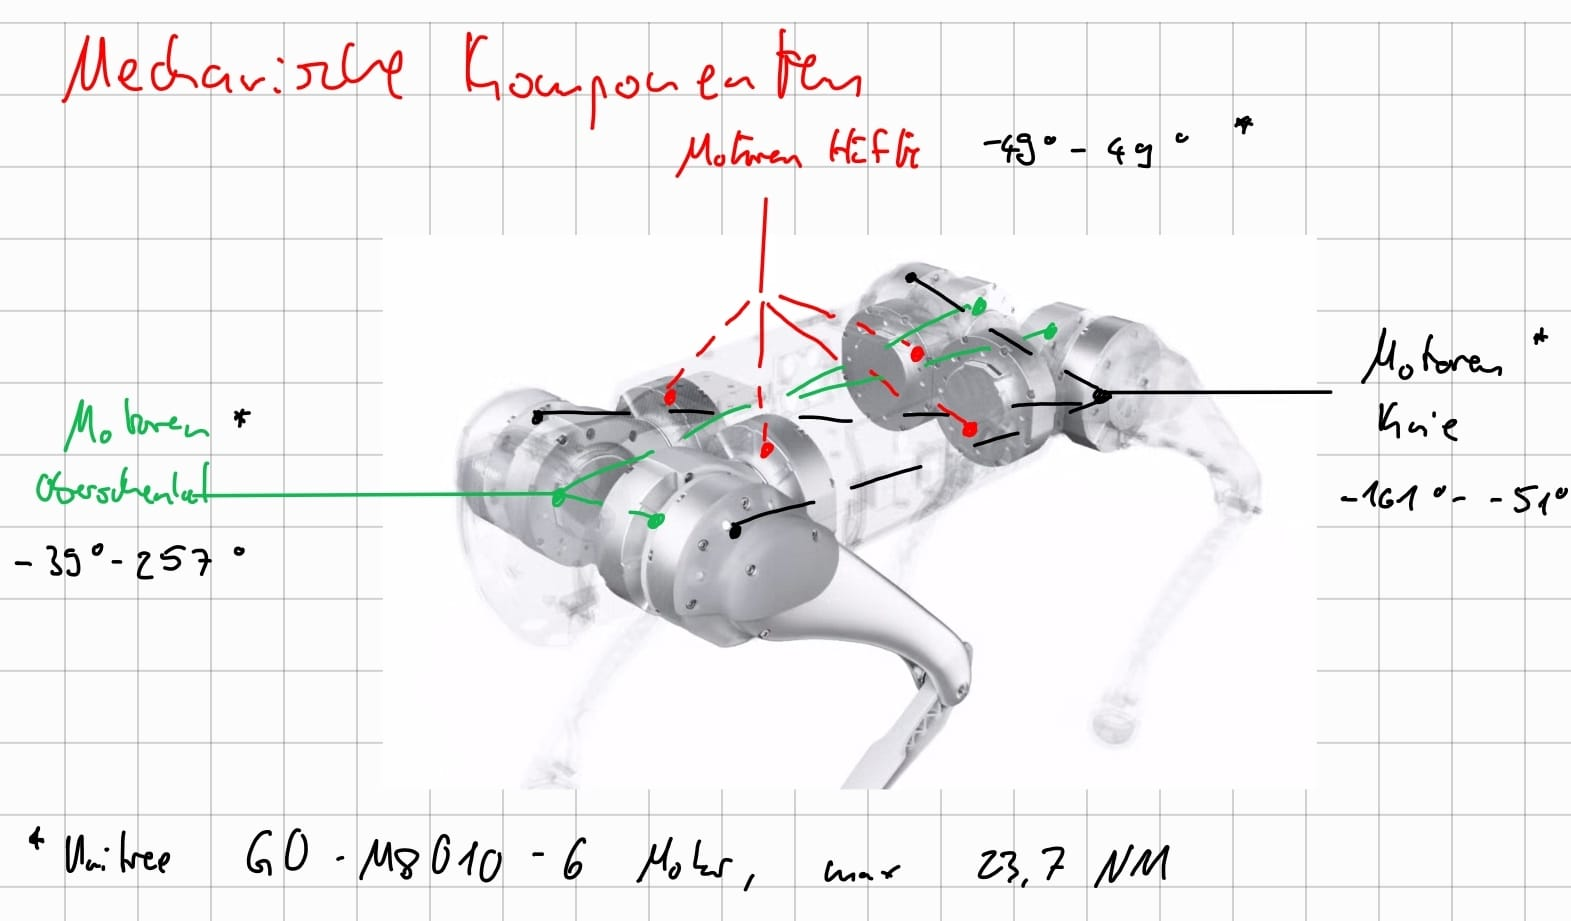
\includegraphics[width=\linewidth]{img/architektur/mechanische_komponenten}}
    \caption[Mechanische Komponenten des Go1]{Mechanische Komponenten des \gls{go1}}\label{fig:mechanische_komponenten}
\end{figure}
Zum Strecken des Kniegelenks wird eine am äußeren Motor angebrachter Seilzug \numref{4} verwendet,
zum Anwinkeln des unteren Beines wir im Gegenzug eine starre Verbindung \numref{5} an der Vorderseite des Kniegelenks genutzt.

\myparagraph{Eigenschaften der Servomotoren}
Die Servomotoren am Hüftgelenk - Abbildung~\ref{fig:mechanische_komponenten}, Bauteil \numref{1}, die Motoren an den Beininnenseiten \numref{2}
und die Motoren an den Beinaußenseiten \numref{3} sind des gleichen Models -
\emph{Unitree Robotics GO-M8010-6 Motor}\footcite{go_motor}.
Die Servomotoren \todo{Sicher Servo?} haben ein maximales Drehmoment von \num{23.7}\gls{nm} und können in 3 verschiedene Konfigurationen
eingeteilt werden:
\begin{enumerate}
    \item \textbf{Hüftmotoren}\\
    Bewegungsradius von \num{-49}\textdegree~bis \num{49}\textdegree
    \item \textbf{Oberschenkelmotoren}\\
    Bewegungsradius von \num{-39}\textdegree~bis \num{257}\textdegree
    \item \textbf{Kniemotoren}\\
    Bewegungsradius von \num{-161}\textdegree~bis \num{-51}\textdegree
\end{enumerate}
Die Motoren sind ebenfalls mit Sensorik bestückt, welche den aktuellen Zustand des Bauteils erkennen und
an die \gls{mcu} schicken können.
Diese Funktionalität wird im Kapitel~\ref{subsubsec:hardware_sensorik} näher beschrieben.

\subsubsection{Hardware und Sensorik}
\label{subsubsec:hardware_sensorik}

Als wichtige Bausteine zur intelligenten Nutzung des \gls{go1} sind an vielen Stellen im Roboter
einige Sensoren oder intelligente Hardware verbaut.
Neben der dedizierten Sensorik zur Erkennung des Umfeldes ist ebenfalls einfachere Sensorik
in einigen Bauteilen wie den mechanischen Bauteilen des Laufapparats verbaut.
Abbildung~\ref{fig:laufapparat} zeigt die hierfür verbauten Sensoren und intelligenten Hardwarebausteine.

\begin{figure}[h]
    \frame{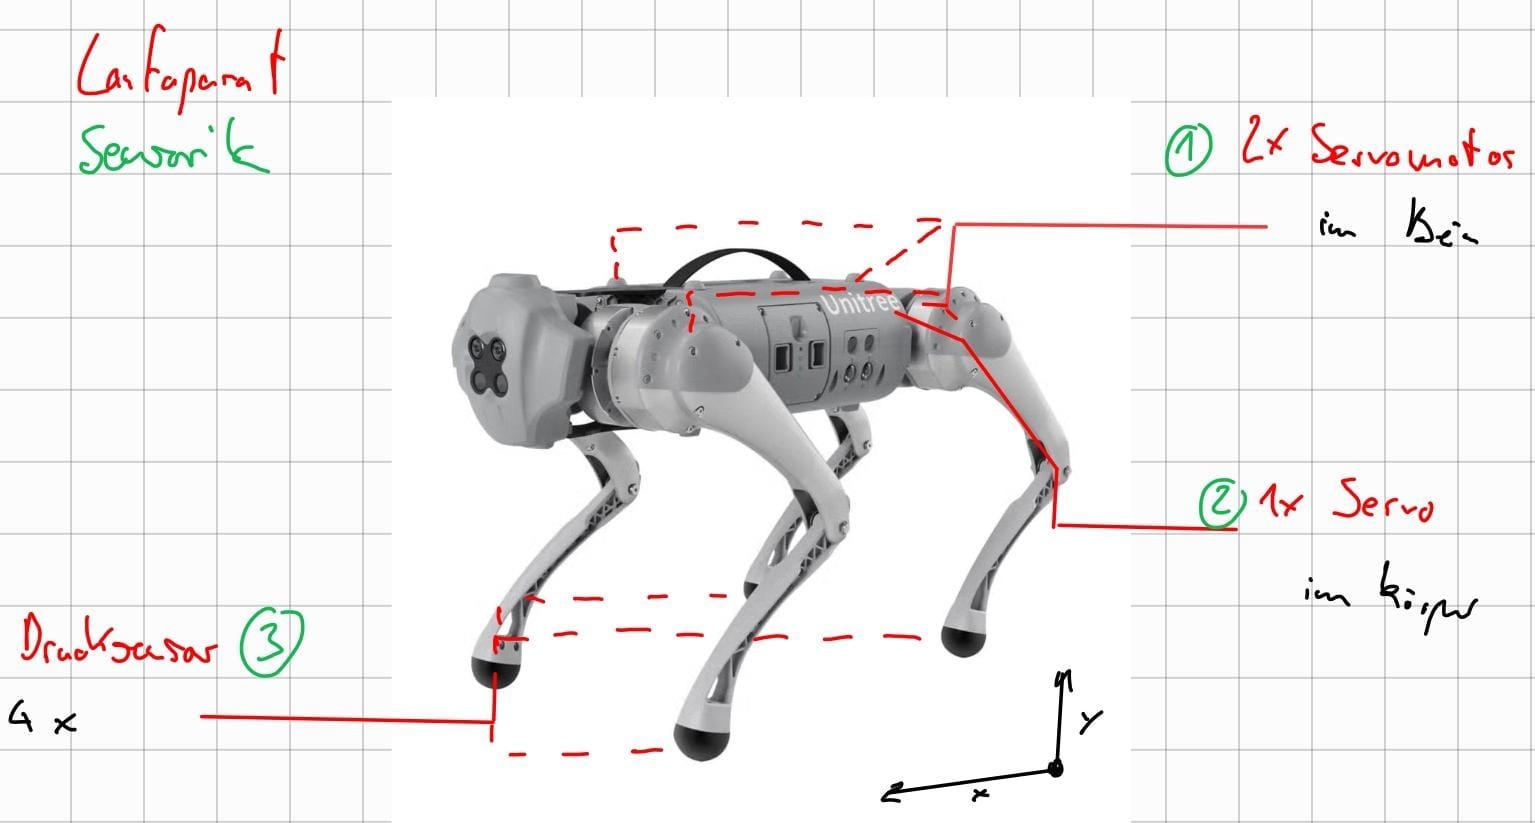
\includegraphics[width=\linewidth]{img/architektur/laufaparat}}
    \caption{Sensorik und Daten des Laufaparats}\label{fig:laufapparat}
\end{figure}

Ähnlich der mechanischen Eigenschaften der zwölf Servomotoren des Typs \emph{GO-M8010-6} - zwei pro Bein des Roboters \numref{1}
und je ein Motor im Körper des Roboters \numref{2} - sind die sensorischen Funktionen dieser identisch.
In Abbildung~\ref{fig:netzwerk_ueberblick} in Kapitel~\ref{subsubsec:netzwerk_ueberblick} ist erkennbar, dass die
zwölf Motoren des \gls{go1} über eine \emph{RS-485} Schnittstelle mit der \gls{mcu} verbunden sind.
Diese wertet die Informationen aus und steuert die einzelnen Motoren über dieselbe Schnittstelle an.

\begin{figure}[h]
    \frame{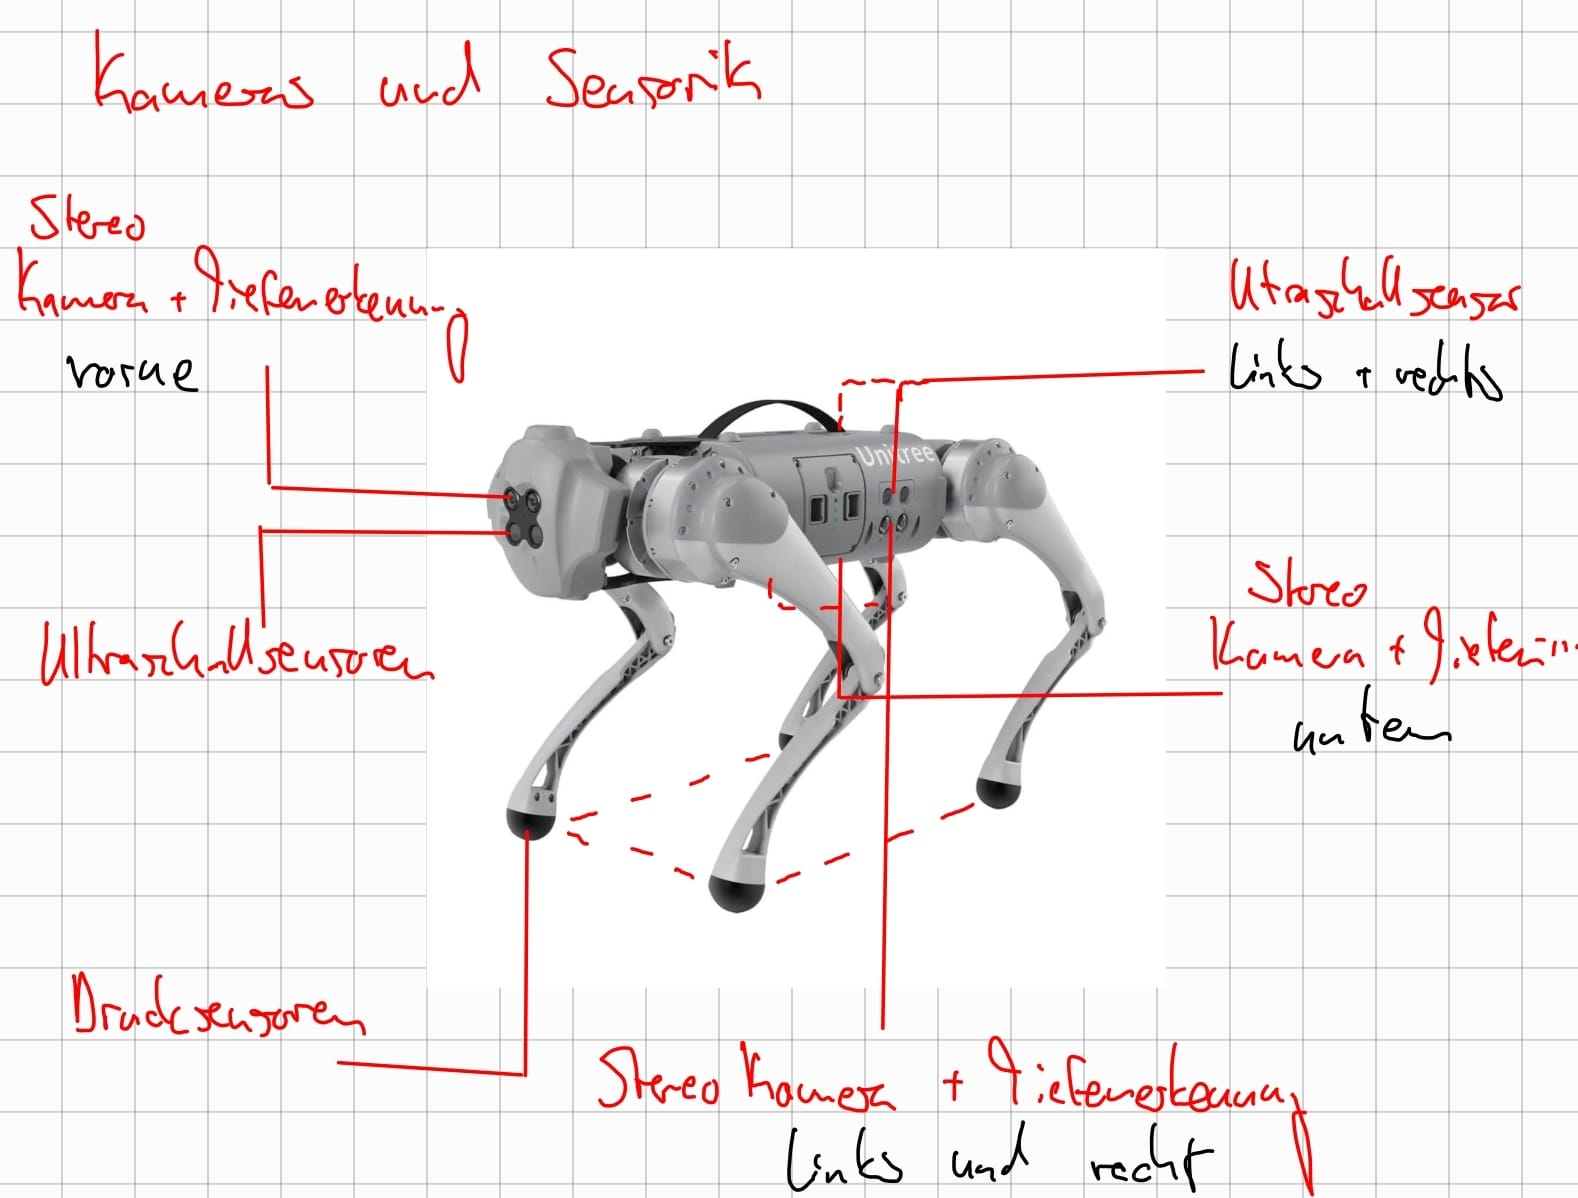
\includegraphics[width=\linewidth]{img/architektur/kameras_sensorik}}
    \caption{Darrstellung der verbauten Kamera und Sensorik}\label{fig:kameras_sensorik}
\end{figure}

\begin{figure}[h]
    \frame{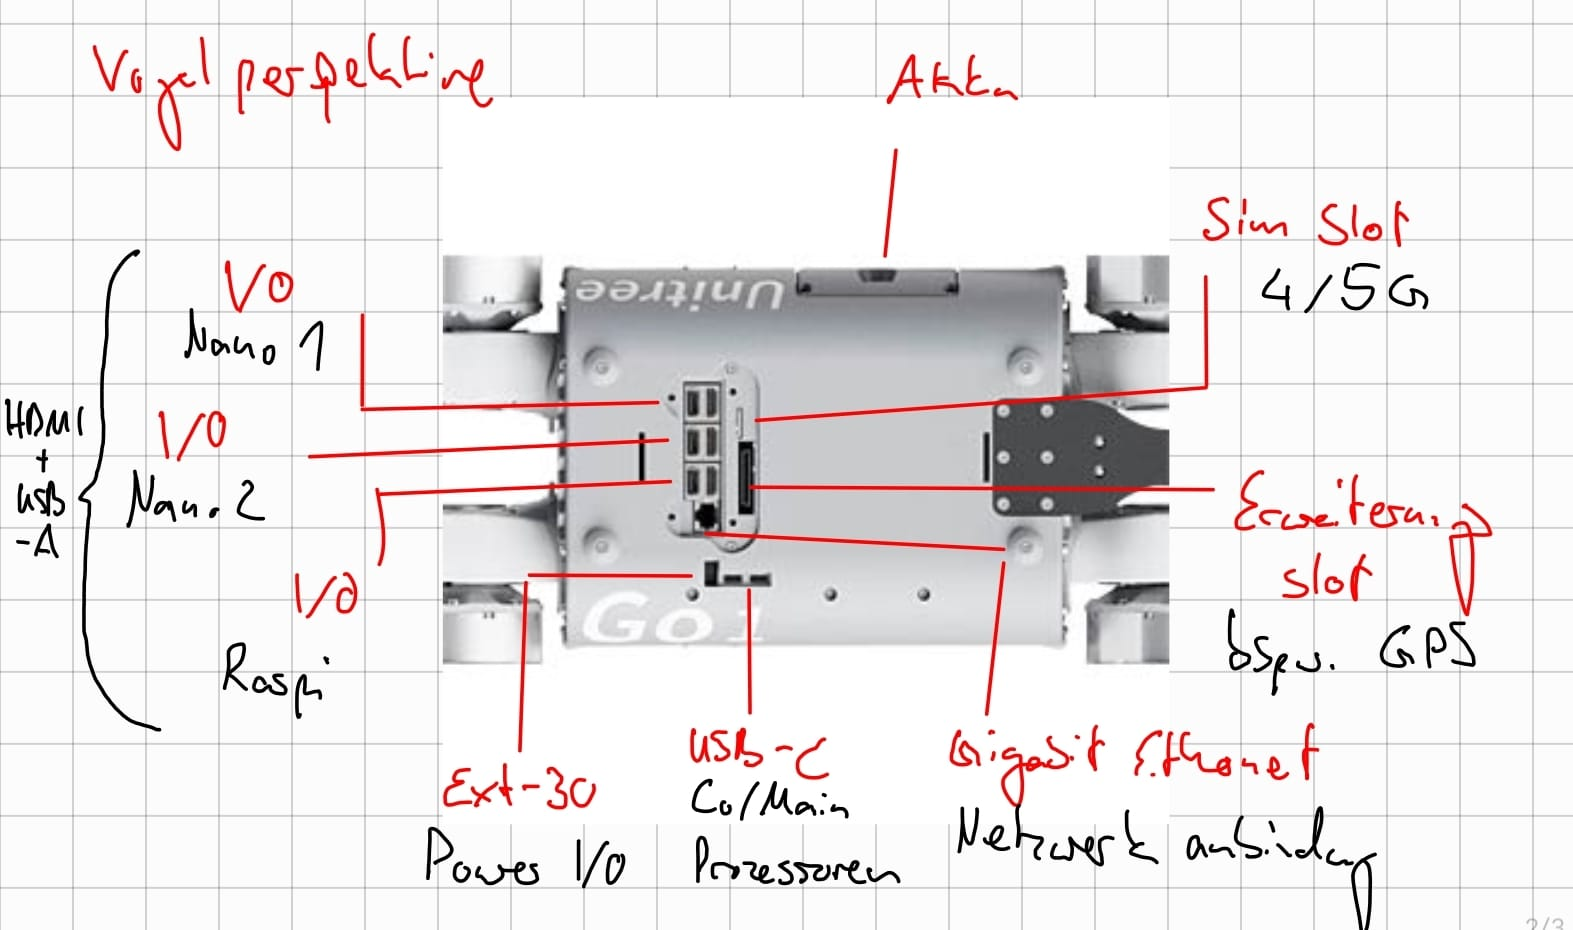
\includegraphics[width=\linewidth]{img/architektur/hardware}}
    \caption{Vogelperspektive mit Hardware}\label{fig:hardware}
\end{figure}
